\documentclass[
  man,
  longtable,
  a4paper,
  nolmodern,
  notxfonts,
  notimes,
  colorlinks=true,linkcolor=blue,citecolor=blue,urlcolor=blue]{apa7}

\usepackage{amsmath}
\usepackage{amssymb}



\usepackage[bidi=default]{babel}
\babelprovide[main,import]{english}


% get rid of language-specific shorthands (see #6817):
\let\LanguageShortHands\languageshorthands
\def\languageshorthands#1{}

\RequirePackage{longtable}
\RequirePackage{threeparttablex}

\makeatletter
\renewcommand{\paragraph}{\@startsection{paragraph}{4}{\parindent}%
	{0\baselineskip \@plus 0.2ex \@minus 0.2ex}%
	{-.5em}%
	{\normalfont\normalsize\bfseries\typesectitle}}

\renewcommand{\subparagraph}[1]{\@startsection{subparagraph}{5}{0.5em}%
	{0\baselineskip \@plus 0.2ex \@minus 0.2ex}%
	{-\z@\relax}%
	{\normalfont\normalsize\bfseries\itshape\hspace{\parindent}{#1}\textit{\addperi}}{\relax}}
\makeatother




\usepackage{longtable, booktabs, multirow, multicol, colortbl, hhline, caption, array, float, xpatch}
\setcounter{topnumber}{2}
\setcounter{bottomnumber}{2}
\setcounter{totalnumber}{4}
\renewcommand{\topfraction}{0.85}
\renewcommand{\bottomfraction}{0.85}
\renewcommand{\textfraction}{0.15}
\renewcommand{\floatpagefraction}{0.7}

\usepackage{tcolorbox}
\tcbuselibrary{listings,theorems, breakable, skins}
\usepackage{fontawesome5}

\definecolor{quarto-callout-color}{HTML}{909090}
\definecolor{quarto-callout-note-color}{HTML}{0758E5}
\definecolor{quarto-callout-important-color}{HTML}{CC1914}
\definecolor{quarto-callout-warning-color}{HTML}{EB9113}
\definecolor{quarto-callout-tip-color}{HTML}{00A047}
\definecolor{quarto-callout-caution-color}{HTML}{FC5300}
\definecolor{quarto-callout-color-frame}{HTML}{ACACAC}
\definecolor{quarto-callout-note-color-frame}{HTML}{4582EC}
\definecolor{quarto-callout-important-color-frame}{HTML}{D9534F}
\definecolor{quarto-callout-warning-color-frame}{HTML}{F0AD4E}
\definecolor{quarto-callout-tip-color-frame}{HTML}{02B875}
\definecolor{quarto-callout-caution-color-frame}{HTML}{FD7E14}

%\newlength\Oldarrayrulewidth
%\newlength\Oldtabcolsep


\usepackage{hyperref}




\providecommand{\tightlist}{%
  \setlength{\itemsep}{0pt}\setlength{\parskip}{0pt}}
\usepackage{longtable,booktabs,array}
\usepackage{calc} % for calculating minipage widths
% Correct order of tables after \paragraph or \subparagraph
\usepackage{etoolbox}
\makeatletter
\patchcmd\longtable{\par}{\if@noskipsec\mbox{}\fi\par}{}{}
\makeatother
% Allow footnotes in longtable head/foot
\IfFileExists{footnotehyper.sty}{\usepackage{footnotehyper}}{\usepackage{footnote}}
\makesavenoteenv{longtable}

\usepackage{graphicx}
\makeatletter
\def\maxwidth{\ifdim\Gin@nat@width>\linewidth\linewidth\else\Gin@nat@width\fi}
\def\maxheight{\ifdim\Gin@nat@height>\textheight\textheight\else\Gin@nat@height\fi}
\makeatother
% Scale images if necessary, so that they will not overflow the page
% margins by default, and it is still possible to overwrite the defaults
% using explicit options in \includegraphics[width, height, ...]{}
\setkeys{Gin}{width=\maxwidth,height=\maxheight,keepaspectratio}
% Set default figure placement to htbp
\makeatletter
\def\fps@figure{htbp}
\makeatother


% definitions for citeproc citations
\NewDocumentCommand\citeproctext{}{}
\NewDocumentCommand\citeproc{mm}{%
  \begingroup\def\citeproctext{#2}\cite{#1}\endgroup}
\makeatletter
 % allow citations to break across lines
 \let\@cite@ofmt\@firstofone
 % avoid brackets around text for \cite:
 \def\@biblabel#1{}
 \def\@cite#1#2{{#1\if@tempswa , #2\fi}}
\makeatother
\newlength{\cslhangindent}
\setlength{\cslhangindent}{1.5em}
\newlength{\csllabelwidth}
\setlength{\csllabelwidth}{3em}
\newenvironment{CSLReferences}[2] % #1 hanging-indent, #2 entry-spacing
 {\begin{list}{}{%
  \setlength{\itemindent}{0pt}
  \setlength{\leftmargin}{0pt}
  \setlength{\parsep}{0pt}
  % turn on hanging indent if param 1 is 1
  \ifodd #1
   \setlength{\leftmargin}{\cslhangindent}
   \setlength{\itemindent}{-1\cslhangindent}
  \fi
  % set entry spacing
  \setlength{\itemsep}{#2\baselineskip}}}
 {\end{list}}
\usepackage{calc}
\newcommand{\CSLBlock}[1]{\hfill\break\parbox[t]{\linewidth}{\strut\ignorespaces#1\strut}}
\newcommand{\CSLLeftMargin}[1]{\parbox[t]{\csllabelwidth}{\strut#1\strut}}
\newcommand{\CSLRightInline}[1]{\parbox[t]{\linewidth - \csllabelwidth}{\strut#1\strut}}
\newcommand{\CSLIndent}[1]{\hspace{\cslhangindent}#1}





\usepackage{newtx}

\defaultfontfeatures{Scale=MatchLowercase}
\defaultfontfeatures[\rmfamily]{Ligatures=TeX,Scale=1}





\title{A Study on Penguins: A Minimal Reproducible Example}


\shorttitle{A Study on Penguins: A Minimal Reproducible Example}


\usepackage{etoolbox}









\authorsnames{Josephine Zerna,Christoph Scheffel}






\authorsaffiliations{
{Faculty of Psychology, Technische Universität Dresden},{}}




\leftheader{Zerna and Scheffel}

\date{2024-08-23}


\abstract{This document is a minimal, reproducible manuscript using the
penguins data set as an example.}

\keywords{penguins, reproducibility, minimal, example}

\authornote{\par{\addORCIDlink{Josephine
Zerna}{0000-0003-2892-884X}}\par{\addORCIDlink{Christoph
Scheffel}{0000-0001-5963-9229}} 

\par{       Author roles were classified using the Contributor Role Taxonomy (CRediT; https://credit.niso.org/) as follows: Josephine
Zerna:   conceptualization, writing; Christoph Scheffel:   project
administration, methodology}
\par{Correspondence concerning this article should be addressed
to Christoph Scheffel, Email: christoph\_scheffel@tu-dresden.de}
}

\makeatletter
\let\endoldlt\endlongtable
\def\endlongtable{
\hline
\endoldlt
}
\makeatother
\RequirePackage{longtable}
\DeclareDelayedFloatFlavor{longtable}{table}

\urlstyle{same}



\usepackage{fontspec}
\usepackage{multirow}
\usepackage{multicol}
\usepackage{colortbl}
\usepackage{hhline}
\newlength\Oldarrayrulewidth
\newlength\Oldtabcolsep
\usepackage{longtable}
\usepackage{array}
\usepackage{hyperref}
\usepackage{float}
\usepackage{wrapfig}
\makeatletter
\@ifpackageloaded{caption}{}{\usepackage{caption}}
\AtBeginDocument{%
\ifdefined\contentsname
  \renewcommand*\contentsname{Table of contents}
\else
  \newcommand\contentsname{Table of contents}
\fi
\ifdefined\listfigurename
  \renewcommand*\listfigurename{List of Figures}
\else
  \newcommand\listfigurename{List of Figures}
\fi
\ifdefined\listtablename
  \renewcommand*\listtablename{List of Tables}
\else
  \newcommand\listtablename{List of Tables}
\fi
\ifdefined\figurename
  \renewcommand*\figurename{Figure}
\else
  \newcommand\figurename{Figure}
\fi
\ifdefined\tablename
  \renewcommand*\tablename{Table}
\else
  \newcommand\tablename{Table}
\fi
}
\@ifpackageloaded{float}{}{\usepackage{float}}
\floatstyle{ruled}
\@ifundefined{c@chapter}{\newfloat{codelisting}{h}{lop}}{\newfloat{codelisting}{h}{lop}[chapter]}
\floatname{codelisting}{Listing}
\newcommand*\listoflistings{\listof{codelisting}{List of Listings}}
\makeatother
\makeatletter
\makeatother
\makeatletter
\@ifpackageloaded{caption}{}{\usepackage{caption}}
\@ifpackageloaded{subcaption}{}{\usepackage{subcaption}}
\makeatother

% From https://tex.stackexchange.com/a/645996/211326
%%% apa7 doesn't want to add appendix section titles in the toc
%%% let's make it do it
\makeatletter
\xpatchcmd{\appendix}
  {\par}
  {\addcontentsline{toc}{section}{\@currentlabelname}\par}
  {}{}
\makeatother

\begin{document}

\maketitle


\setcounter{secnumdepth}{-\maxdimen} % remove section numbering

\setlength\LTleft{0pt}


\section{Introduction}\label{introduction}

Penguins are fascinating creatures that inhabit various regions of the
Southern Hemisphere, including Antarctica and surrounding islands. The
study of penguins provides valuable insights into ecosystem dynamics,
climate change impacts, and evolutionary biology
(\citeproc{ref-jones2018}{Jones, 2018}; \citeproc{ref-smith2020}{Smith,
2020}).

This manuscript presents a minimal reproducible example utilizing the
penguins dataset to demonstrate scientific workflows in R.

\section{Methods}\label{methods}

We conducted a two-sample Welch \emph{t}-test to compare the average
bill lengths between male and female penguins. The null hypothesis
(\(H_0\)) states that there is no difference in bill lengths between
male and female penguins, while the alternative hypothesis (\(H_1\))
suggests a significant difference.

The \emph{t}-test was performed using the \texttt{t.test()} function in
R, with a significance level of 0.05.

\section{Results}\label{results}

Descriptive statistics of the data set are given in
Table~\ref{tbl-descriptive-statistics} and individual bill lengths are
displayed in Figure~\ref{fig-bill-length-comparison}.

\begin{table}

{\caption{{Descriptive Statistics}{\label{tbl-descriptive-statistics}}}
\vspace{-20pt}}

\global\setlength{\Oldarrayrulewidth}{\arrayrulewidth}

\global\setlength{\Oldtabcolsep}{\tabcolsep}

\setlength{\tabcolsep}{2pt}

\renewcommand*{\arraystretch}{1.5}



\providecommand{\ascline}[3]{\noalign{\global\arrayrulewidth #1}\arrayrulecolor[HTML]{#2}\cline{#3}}

\begin{longtable*}[c]{|p{0.75in}|p{0.75in}|p{0.75in}|p{0.75in}|p{0.75in}|p{0.75in}|p{0.75in}|p{0.75in}}



\ascline{0.75pt}{000000}{1-8}

\multicolumn{2}{>{\centering}m{\dimexpr 1.5in+2\tabcolsep}}{\textcolor[HTML]{000000}{\fontsize{11}{22}\selectfont{\global\setmainfont{TeX Gyre Termes}{\ }}}} & \multicolumn{2}{>{\centering}m{\dimexpr 1.5in+2\tabcolsep}}{\textcolor[HTML]{000000}{\fontsize{11}{22}\selectfont{\global\setmainfont{TeX Gyre Termes}{female\ (N=165)}}}} & \multicolumn{2}{>{\centering}m{\dimexpr 1.5in+2\tabcolsep}}{\textcolor[HTML]{000000}{\fontsize{11}{22}\selectfont{\global\setmainfont{TeX Gyre Termes}{male\ (N=168)}}}} & \multicolumn{2}{>{\centering}m{\dimexpr 1.5in+2\tabcolsep}}{\textcolor[HTML]{000000}{\fontsize{11}{22}\selectfont{\global\setmainfont{TeX Gyre Termes}{unknown\ (N=11)}}}} \\

\ascline{1.5pt}{666666}{1-8}



\multicolumn{1}{>{\centering}m{\dimexpr 0.75in+0\tabcolsep}}{\textcolor[HTML]{000000}{\fontsize{11}{22}\selectfont{\global\setmainfont{TeX Gyre Termes}{\ }}}} & \multicolumn{1}{>{\centering}m{\dimexpr 0.75in+0\tabcolsep}}{\textcolor[HTML]{000000}{\fontsize{11}{22}\selectfont{\global\setmainfont{TeX Gyre Termes}{\ \ }}}} & \multicolumn{1}{>{\centering}m{\dimexpr 0.75in+0\tabcolsep}}{\textcolor[HTML]{000000}{\fontsize{11}{22}\selectfont{\global\setmainfont{TeX Gyre Termes}{Mean}}}} & \multicolumn{1}{>{\centering}m{\dimexpr 0.75in+0\tabcolsep}}{\textcolor[HTML]{000000}{\fontsize{11}{22}\selectfont{\global\setmainfont{TeX Gyre Termes}{Std.\ Dev.}}}} & \multicolumn{1}{>{\centering}m{\dimexpr 0.75in+0\tabcolsep}}{\textcolor[HTML]{000000}{\fontsize{11}{22}\selectfont{\global\setmainfont{TeX Gyre Termes}{Mean\ }}}} & \multicolumn{1}{>{\centering}m{\dimexpr 0.75in+0\tabcolsep}}{\textcolor[HTML]{000000}{\fontsize{11}{22}\selectfont{\global\setmainfont{TeX Gyre Termes}{Std.\ Dev.\ }}}} & \multicolumn{1}{>{\centering}m{\dimexpr 0.75in+0\tabcolsep}}{\textcolor[HTML]{000000}{\fontsize{11}{22}\selectfont{\global\setmainfont{TeX Gyre Termes}{Mean\ \ }}}} & \multicolumn{1}{>{\centering}m{\dimexpr 0.75in+0\tabcolsep}}{\textcolor[HTML]{000000}{\fontsize{11}{22}\selectfont{\global\setmainfont{TeX Gyre Termes}{Std.\ Dev.\ \ }}}} \\

\ascline{0.75pt}{000000}{1-8}\endfirsthead 

\ascline{0.75pt}{000000}{1-8}

\multicolumn{2}{>{\centering}m{\dimexpr 1.5in+2\tabcolsep}}{\textcolor[HTML]{000000}{\fontsize{11}{22}\selectfont{\global\setmainfont{TeX Gyre Termes}{\ }}}} & \multicolumn{2}{>{\centering}m{\dimexpr 1.5in+2\tabcolsep}}{\textcolor[HTML]{000000}{\fontsize{11}{22}\selectfont{\global\setmainfont{TeX Gyre Termes}{female\ (N=165)}}}} & \multicolumn{2}{>{\centering}m{\dimexpr 1.5in+2\tabcolsep}}{\textcolor[HTML]{000000}{\fontsize{11}{22}\selectfont{\global\setmainfont{TeX Gyre Termes}{male\ (N=168)}}}} & \multicolumn{2}{>{\centering}m{\dimexpr 1.5in+2\tabcolsep}}{\textcolor[HTML]{000000}{\fontsize{11}{22}\selectfont{\global\setmainfont{TeX Gyre Termes}{unknown\ (N=11)}}}} \\

\ascline{1.5pt}{666666}{1-8}



\multicolumn{1}{>{\centering}m{\dimexpr 0.75in+0\tabcolsep}}{\textcolor[HTML]{000000}{\fontsize{11}{22}\selectfont{\global\setmainfont{TeX Gyre Termes}{\ }}}} & \multicolumn{1}{>{\centering}m{\dimexpr 0.75in+0\tabcolsep}}{\textcolor[HTML]{000000}{\fontsize{11}{22}\selectfont{\global\setmainfont{TeX Gyre Termes}{\ \ }}}} & \multicolumn{1}{>{\centering}m{\dimexpr 0.75in+0\tabcolsep}}{\textcolor[HTML]{000000}{\fontsize{11}{22}\selectfont{\global\setmainfont{TeX Gyre Termes}{Mean}}}} & \multicolumn{1}{>{\centering}m{\dimexpr 0.75in+0\tabcolsep}}{\textcolor[HTML]{000000}{\fontsize{11}{22}\selectfont{\global\setmainfont{TeX Gyre Termes}{Std.\ Dev.}}}} & \multicolumn{1}{>{\centering}m{\dimexpr 0.75in+0\tabcolsep}}{\textcolor[HTML]{000000}{\fontsize{11}{22}\selectfont{\global\setmainfont{TeX Gyre Termes}{Mean\ }}}} & \multicolumn{1}{>{\centering}m{\dimexpr 0.75in+0\tabcolsep}}{\textcolor[HTML]{000000}{\fontsize{11}{22}\selectfont{\global\setmainfont{TeX Gyre Termes}{Std.\ Dev.\ }}}} & \multicolumn{1}{>{\centering}m{\dimexpr 0.75in+0\tabcolsep}}{\textcolor[HTML]{000000}{\fontsize{11}{22}\selectfont{\global\setmainfont{TeX Gyre Termes}{Mean\ \ }}}} & \multicolumn{1}{>{\centering}m{\dimexpr 0.75in+0\tabcolsep}}{\textcolor[HTML]{000000}{\fontsize{11}{22}\selectfont{\global\setmainfont{TeX Gyre Termes}{Std.\ Dev.\ \ }}}} \\

\ascline{0.75pt}{000000}{1-8}\endhead



\multicolumn{1}{>{\centering}m{\dimexpr 0.75in+0\tabcolsep}}{\textcolor[HTML]{000000}{\fontsize{11}{22}\selectfont{\global\setmainfont{TeX Gyre Termes}{bill\_length\_mm\ (N=342)}}}} & \multicolumn{1}{>{\centering}m{\dimexpr 0.75in+0\tabcolsep}}{\textcolor[HTML]{000000}{\fontsize{11}{22}\selectfont{\global\setmainfont{TeX Gyre Termes}{}}}} & \multicolumn{1}{>{\centering}m{\dimexpr 0.75in+0\tabcolsep}}{\textcolor[HTML]{000000}{\fontsize{11}{22}\selectfont{\global\setmainfont{TeX Gyre Termes}{42.1}}}} & \multicolumn{1}{>{\centering}m{\dimexpr 0.75in+0\tabcolsep}}{\textcolor[HTML]{000000}{\fontsize{11}{22}\selectfont{\global\setmainfont{TeX Gyre Termes}{4.9}}}} & \multicolumn{1}{>{\centering}m{\dimexpr 0.75in+0\tabcolsep}}{\textcolor[HTML]{000000}{\fontsize{11}{22}\selectfont{\global\setmainfont{TeX Gyre Termes}{45.9}}}} & \multicolumn{1}{>{\centering}m{\dimexpr 0.75in+0\tabcolsep}}{\textcolor[HTML]{000000}{\fontsize{11}{22}\selectfont{\global\setmainfont{TeX Gyre Termes}{5.4}}}} & \multicolumn{1}{>{\centering}m{\dimexpr 0.75in+0\tabcolsep}}{\textcolor[HTML]{000000}{\fontsize{11}{22}\selectfont{\global\setmainfont{TeX Gyre Termes}{41.3}}}} & \multicolumn{1}{>{\centering}m{\dimexpr 0.75in+0\tabcolsep}}{\textcolor[HTML]{000000}{\fontsize{11}{22}\selectfont{\global\setmainfont{TeX Gyre Termes}{4.6}}}} \\





\multicolumn{1}{>{\centering}m{\dimexpr 0.75in+0\tabcolsep}}{\textcolor[HTML]{000000}{\fontsize{11}{22}\selectfont{\global\setmainfont{TeX Gyre Termes}{bill\_depth\_mm\ (N=342)}}}} & \multicolumn{1}{>{\centering}m{\dimexpr 0.75in+0\tabcolsep}}{\textcolor[HTML]{000000}{\fontsize{11}{22}\selectfont{\global\setmainfont{TeX Gyre Termes}{}}}} & \multicolumn{1}{>{\centering}m{\dimexpr 0.75in+0\tabcolsep}}{\textcolor[HTML]{000000}{\fontsize{11}{22}\selectfont{\global\setmainfont{TeX Gyre Termes}{16.4}}}} & \multicolumn{1}{>{\centering}m{\dimexpr 0.75in+0\tabcolsep}}{\textcolor[HTML]{000000}{\fontsize{11}{22}\selectfont{\global\setmainfont{TeX Gyre Termes}{1.8}}}} & \multicolumn{1}{>{\centering}m{\dimexpr 0.75in+0\tabcolsep}}{\textcolor[HTML]{000000}{\fontsize{11}{22}\selectfont{\global\setmainfont{TeX Gyre Termes}{17.9}}}} & \multicolumn{1}{>{\centering}m{\dimexpr 0.75in+0\tabcolsep}}{\textcolor[HTML]{000000}{\fontsize{11}{22}\selectfont{\global\setmainfont{TeX Gyre Termes}{1.9}}}} & \multicolumn{1}{>{\centering}m{\dimexpr 0.75in+0\tabcolsep}}{\textcolor[HTML]{000000}{\fontsize{11}{22}\selectfont{\global\setmainfont{TeX Gyre Termes}{16.6}}}} & \multicolumn{1}{>{\centering}m{\dimexpr 0.75in+0\tabcolsep}}{\textcolor[HTML]{000000}{\fontsize{11}{22}\selectfont{\global\setmainfont{TeX Gyre Termes}{2.2}}}} \\





\multicolumn{1}{>{\centering}m{\dimexpr 0.75in+0\tabcolsep}}{\textcolor[HTML]{000000}{\fontsize{11}{22}\selectfont{\global\setmainfont{TeX Gyre Termes}{flipper\_length\_mm\ (N=342)}}}} & \multicolumn{1}{>{\centering}m{\dimexpr 0.75in+0\tabcolsep}}{\textcolor[HTML]{000000}{\fontsize{11}{22}\selectfont{\global\setmainfont{TeX Gyre Termes}{}}}} & \multicolumn{1}{>{\centering}m{\dimexpr 0.75in+0\tabcolsep}}{\textcolor[HTML]{000000}{\fontsize{11}{22}\selectfont{\global\setmainfont{TeX Gyre Termes}{197.4}}}} & \multicolumn{1}{>{\centering}m{\dimexpr 0.75in+0\tabcolsep}}{\textcolor[HTML]{000000}{\fontsize{11}{22}\selectfont{\global\setmainfont{TeX Gyre Termes}{12.5}}}} & \multicolumn{1}{>{\centering}m{\dimexpr 0.75in+0\tabcolsep}}{\textcolor[HTML]{000000}{\fontsize{11}{22}\selectfont{\global\setmainfont{TeX Gyre Termes}{204.5}}}} & \multicolumn{1}{>{\centering}m{\dimexpr 0.75in+0\tabcolsep}}{\textcolor[HTML]{000000}{\fontsize{11}{22}\selectfont{\global\setmainfont{TeX Gyre Termes}{14.5}}}} & \multicolumn{1}{>{\centering}m{\dimexpr 0.75in+0\tabcolsep}}{\textcolor[HTML]{000000}{\fontsize{11}{22}\selectfont{\global\setmainfont{TeX Gyre Termes}{199.0}}}} & \multicolumn{1}{>{\centering}m{\dimexpr 0.75in+0\tabcolsep}}{\textcolor[HTML]{000000}{\fontsize{11}{22}\selectfont{\global\setmainfont{TeX Gyre Termes}{16.5}}}} \\





\multicolumn{1}{>{\centering}m{\dimexpr 0.75in+0\tabcolsep}}{\textcolor[HTML]{000000}{\fontsize{11}{22}\selectfont{\global\setmainfont{TeX Gyre Termes}{body\_mass\_g\ (N=342)}}}} & \multicolumn{1}{>{\centering}m{\dimexpr 0.75in+0\tabcolsep}}{\textcolor[HTML]{000000}{\fontsize{11}{22}\selectfont{\global\setmainfont{TeX Gyre Termes}{}}}} & \multicolumn{1}{>{\centering}m{\dimexpr 0.75in+0\tabcolsep}}{\textcolor[HTML]{000000}{\fontsize{11}{22}\selectfont{\global\setmainfont{TeX Gyre Termes}{3862.3}}}} & \multicolumn{1}{>{\centering}m{\dimexpr 0.75in+0\tabcolsep}}{\textcolor[HTML]{000000}{\fontsize{11}{22}\selectfont{\global\setmainfont{TeX Gyre Termes}{666.2}}}} & \multicolumn{1}{>{\centering}m{\dimexpr 0.75in+0\tabcolsep}}{\textcolor[HTML]{000000}{\fontsize{11}{22}\selectfont{\global\setmainfont{TeX Gyre Termes}{4545.7}}}} & \multicolumn{1}{>{\centering}m{\dimexpr 0.75in+0\tabcolsep}}{\textcolor[HTML]{000000}{\fontsize{11}{22}\selectfont{\global\setmainfont{TeX Gyre Termes}{787.6}}}} & \multicolumn{1}{>{\centering}m{\dimexpr 0.75in+0\tabcolsep}}{\textcolor[HTML]{000000}{\fontsize{11}{22}\selectfont{\global\setmainfont{TeX Gyre Termes}{4005.6}}}} & \multicolumn{1}{>{\centering}m{\dimexpr 0.75in+0\tabcolsep}}{\textcolor[HTML]{000000}{\fontsize{11}{22}\selectfont{\global\setmainfont{TeX Gyre Termes}{679.4}}}} \\

\ascline{1pt}{000000}{1-8}



\multicolumn{1}{>{\centering}m{\dimexpr 0.75in+0\tabcolsep}}{\textcolor[HTML]{000000}{\fontsize{11}{22}\selectfont{\global\setmainfont{TeX Gyre Termes}{}}}} & \multicolumn{1}{>{\centering}m{\dimexpr 0.75in+0\tabcolsep}}{\textcolor[HTML]{000000}{\fontsize{11}{22}\selectfont{\global\setmainfont{TeX Gyre Termes}{}}}} & \multicolumn{1}{>{\centering}m{\dimexpr 0.75in+0\tabcolsep}}{\textcolor[HTML]{000000}{\fontsize{11}{22}\selectfont{\global\setmainfont{TeX Gyre Termes}{N}}}} & \multicolumn{1}{>{\centering}m{\dimexpr 0.75in+0\tabcolsep}}{\textcolor[HTML]{000000}{\fontsize{11}{22}\selectfont{\global\setmainfont{TeX Gyre Termes}{Pct.}}}} & \multicolumn{1}{>{\centering}m{\dimexpr 0.75in+0\tabcolsep}}{\textcolor[HTML]{000000}{\fontsize{11}{22}\selectfont{\global\setmainfont{TeX Gyre Termes}{N}}}} & \multicolumn{1}{>{\centering}m{\dimexpr 0.75in+0\tabcolsep}}{\textcolor[HTML]{000000}{\fontsize{11}{22}\selectfont{\global\setmainfont{TeX Gyre Termes}{Pct.}}}} & \multicolumn{1}{>{\centering}m{\dimexpr 0.75in+0\tabcolsep}}{\textcolor[HTML]{000000}{\fontsize{11}{22}\selectfont{\global\setmainfont{TeX Gyre Termes}{N}}}} & \multicolumn{1}{>{\centering}m{\dimexpr 0.75in+0\tabcolsep}}{\textcolor[HTML]{000000}{\fontsize{11}{22}\selectfont{\global\setmainfont{TeX Gyre Termes}{Pct.}}}} \\





\multicolumn{1}{>{\centering}m{\dimexpr 0.75in+0\tabcolsep}}{\textcolor[HTML]{000000}{\fontsize{11}{22}\selectfont{\global\setmainfont{TeX Gyre Termes}{species}}}} & \multicolumn{1}{>{\centering}m{\dimexpr 0.75in+0\tabcolsep}}{\textcolor[HTML]{000000}{\fontsize{11}{22}\selectfont{\global\setmainfont{TeX Gyre Termes}{Adelie}}}} & \multicolumn{1}{>{\centering}m{\dimexpr 0.75in+0\tabcolsep}}{\textcolor[HTML]{000000}{\fontsize{11}{22}\selectfont{\global\setmainfont{TeX Gyre Termes}{73}}}} & \multicolumn{1}{>{\centering}m{\dimexpr 0.75in+0\tabcolsep}}{\textcolor[HTML]{000000}{\fontsize{11}{22}\selectfont{\global\setmainfont{TeX Gyre Termes}{44.2}}}} & \multicolumn{1}{>{\centering}m{\dimexpr 0.75in+0\tabcolsep}}{\textcolor[HTML]{000000}{\fontsize{11}{22}\selectfont{\global\setmainfont{TeX Gyre Termes}{73}}}} & \multicolumn{1}{>{\centering}m{\dimexpr 0.75in+0\tabcolsep}}{\textcolor[HTML]{000000}{\fontsize{11}{22}\selectfont{\global\setmainfont{TeX Gyre Termes}{43.5}}}} & \multicolumn{1}{>{\centering}m{\dimexpr 0.75in+0\tabcolsep}}{\textcolor[HTML]{000000}{\fontsize{11}{22}\selectfont{\global\setmainfont{TeX Gyre Termes}{6}}}} & \multicolumn{1}{>{\centering}m{\dimexpr 0.75in+0\tabcolsep}}{\textcolor[HTML]{000000}{\fontsize{11}{22}\selectfont{\global\setmainfont{TeX Gyre Termes}{54.5}}}} \\





\multicolumn{1}{>{\centering}m{\dimexpr 0.75in+0\tabcolsep}}{\textcolor[HTML]{000000}{\fontsize{11}{22}\selectfont{\global\setmainfont{TeX Gyre Termes}{}}}} & \multicolumn{1}{>{\centering}m{\dimexpr 0.75in+0\tabcolsep}}{\textcolor[HTML]{000000}{\fontsize{11}{22}\selectfont{\global\setmainfont{TeX Gyre Termes}{Chinstrap}}}} & \multicolumn{1}{>{\centering}m{\dimexpr 0.75in+0\tabcolsep}}{\textcolor[HTML]{000000}{\fontsize{11}{22}\selectfont{\global\setmainfont{TeX Gyre Termes}{34}}}} & \multicolumn{1}{>{\centering}m{\dimexpr 0.75in+0\tabcolsep}}{\textcolor[HTML]{000000}{\fontsize{11}{22}\selectfont{\global\setmainfont{TeX Gyre Termes}{20.6}}}} & \multicolumn{1}{>{\centering}m{\dimexpr 0.75in+0\tabcolsep}}{\textcolor[HTML]{000000}{\fontsize{11}{22}\selectfont{\global\setmainfont{TeX Gyre Termes}{34}}}} & \multicolumn{1}{>{\centering}m{\dimexpr 0.75in+0\tabcolsep}}{\textcolor[HTML]{000000}{\fontsize{11}{22}\selectfont{\global\setmainfont{TeX Gyre Termes}{20.2}}}} & \multicolumn{1}{>{\centering}m{\dimexpr 0.75in+0\tabcolsep}}{\textcolor[HTML]{000000}{\fontsize{11}{22}\selectfont{\global\setmainfont{TeX Gyre Termes}{0}}}} & \multicolumn{1}{>{\centering}m{\dimexpr 0.75in+0\tabcolsep}}{\textcolor[HTML]{000000}{\fontsize{11}{22}\selectfont{\global\setmainfont{TeX Gyre Termes}{0.0}}}} \\





\multicolumn{1}{>{\centering}m{\dimexpr 0.75in+0\tabcolsep}}{\textcolor[HTML]{000000}{\fontsize{11}{22}\selectfont{\global\setmainfont{TeX Gyre Termes}{}}}} & \multicolumn{1}{>{\centering}m{\dimexpr 0.75in+0\tabcolsep}}{\textcolor[HTML]{000000}{\fontsize{11}{22}\selectfont{\global\setmainfont{TeX Gyre Termes}{Gentoo}}}} & \multicolumn{1}{>{\centering}m{\dimexpr 0.75in+0\tabcolsep}}{\textcolor[HTML]{000000}{\fontsize{11}{22}\selectfont{\global\setmainfont{TeX Gyre Termes}{58}}}} & \multicolumn{1}{>{\centering}m{\dimexpr 0.75in+0\tabcolsep}}{\textcolor[HTML]{000000}{\fontsize{11}{22}\selectfont{\global\setmainfont{TeX Gyre Termes}{35.2}}}} & \multicolumn{1}{>{\centering}m{\dimexpr 0.75in+0\tabcolsep}}{\textcolor[HTML]{000000}{\fontsize{11}{22}\selectfont{\global\setmainfont{TeX Gyre Termes}{61}}}} & \multicolumn{1}{>{\centering}m{\dimexpr 0.75in+0\tabcolsep}}{\textcolor[HTML]{000000}{\fontsize{11}{22}\selectfont{\global\setmainfont{TeX Gyre Termes}{36.3}}}} & \multicolumn{1}{>{\centering}m{\dimexpr 0.75in+0\tabcolsep}}{\textcolor[HTML]{000000}{\fontsize{11}{22}\selectfont{\global\setmainfont{TeX Gyre Termes}{5}}}} & \multicolumn{1}{>{\centering}m{\dimexpr 0.75in+0\tabcolsep}}{\textcolor[HTML]{000000}{\fontsize{11}{22}\selectfont{\global\setmainfont{TeX Gyre Termes}{45.5}}}} \\





\multicolumn{1}{>{\centering}m{\dimexpr 0.75in+0\tabcolsep}}{\textcolor[HTML]{000000}{\fontsize{11}{22}\selectfont{\global\setmainfont{TeX Gyre Termes}{island}}}} & \multicolumn{1}{>{\centering}m{\dimexpr 0.75in+0\tabcolsep}}{\textcolor[HTML]{000000}{\fontsize{11}{22}\selectfont{\global\setmainfont{TeX Gyre Termes}{Biscoe}}}} & \multicolumn{1}{>{\centering}m{\dimexpr 0.75in+0\tabcolsep}}{\textcolor[HTML]{000000}{\fontsize{11}{22}\selectfont{\global\setmainfont{TeX Gyre Termes}{80}}}} & \multicolumn{1}{>{\centering}m{\dimexpr 0.75in+0\tabcolsep}}{\textcolor[HTML]{000000}{\fontsize{11}{22}\selectfont{\global\setmainfont{TeX Gyre Termes}{48.5}}}} & \multicolumn{1}{>{\centering}m{\dimexpr 0.75in+0\tabcolsep}}{\textcolor[HTML]{000000}{\fontsize{11}{22}\selectfont{\global\setmainfont{TeX Gyre Termes}{83}}}} & \multicolumn{1}{>{\centering}m{\dimexpr 0.75in+0\tabcolsep}}{\textcolor[HTML]{000000}{\fontsize{11}{22}\selectfont{\global\setmainfont{TeX Gyre Termes}{49.4}}}} & \multicolumn{1}{>{\centering}m{\dimexpr 0.75in+0\tabcolsep}}{\textcolor[HTML]{000000}{\fontsize{11}{22}\selectfont{\global\setmainfont{TeX Gyre Termes}{5}}}} & \multicolumn{1}{>{\centering}m{\dimexpr 0.75in+0\tabcolsep}}{\textcolor[HTML]{000000}{\fontsize{11}{22}\selectfont{\global\setmainfont{TeX Gyre Termes}{45.5}}}} \\





\multicolumn{1}{>{\centering}m{\dimexpr 0.75in+0\tabcolsep}}{\textcolor[HTML]{000000}{\fontsize{11}{22}\selectfont{\global\setmainfont{TeX Gyre Termes}{}}}} & \multicolumn{1}{>{\centering}m{\dimexpr 0.75in+0\tabcolsep}}{\textcolor[HTML]{000000}{\fontsize{11}{22}\selectfont{\global\setmainfont{TeX Gyre Termes}{Dream}}}} & \multicolumn{1}{>{\centering}m{\dimexpr 0.75in+0\tabcolsep}}{\textcolor[HTML]{000000}{\fontsize{11}{22}\selectfont{\global\setmainfont{TeX Gyre Termes}{61}}}} & \multicolumn{1}{>{\centering}m{\dimexpr 0.75in+0\tabcolsep}}{\textcolor[HTML]{000000}{\fontsize{11}{22}\selectfont{\global\setmainfont{TeX Gyre Termes}{37.0}}}} & \multicolumn{1}{>{\centering}m{\dimexpr 0.75in+0\tabcolsep}}{\textcolor[HTML]{000000}{\fontsize{11}{22}\selectfont{\global\setmainfont{TeX Gyre Termes}{62}}}} & \multicolumn{1}{>{\centering}m{\dimexpr 0.75in+0\tabcolsep}}{\textcolor[HTML]{000000}{\fontsize{11}{22}\selectfont{\global\setmainfont{TeX Gyre Termes}{36.9}}}} & \multicolumn{1}{>{\centering}m{\dimexpr 0.75in+0\tabcolsep}}{\textcolor[HTML]{000000}{\fontsize{11}{22}\selectfont{\global\setmainfont{TeX Gyre Termes}{1}}}} & \multicolumn{1}{>{\centering}m{\dimexpr 0.75in+0\tabcolsep}}{\textcolor[HTML]{000000}{\fontsize{11}{22}\selectfont{\global\setmainfont{TeX Gyre Termes}{9.1}}}} \\





\multicolumn{1}{>{\centering}m{\dimexpr 0.75in+0\tabcolsep}}{\textcolor[HTML]{000000}{\fontsize{11}{22}\selectfont{\global\setmainfont{TeX Gyre Termes}{}}}} & \multicolumn{1}{>{\centering}m{\dimexpr 0.75in+0\tabcolsep}}{\textcolor[HTML]{000000}{\fontsize{11}{22}\selectfont{\global\setmainfont{TeX Gyre Termes}{Torgersen}}}} & \multicolumn{1}{>{\centering}m{\dimexpr 0.75in+0\tabcolsep}}{\textcolor[HTML]{000000}{\fontsize{11}{22}\selectfont{\global\setmainfont{TeX Gyre Termes}{24}}}} & \multicolumn{1}{>{\centering}m{\dimexpr 0.75in+0\tabcolsep}}{\textcolor[HTML]{000000}{\fontsize{11}{22}\selectfont{\global\setmainfont{TeX Gyre Termes}{14.5}}}} & \multicolumn{1}{>{\centering}m{\dimexpr 0.75in+0\tabcolsep}}{\textcolor[HTML]{000000}{\fontsize{11}{22}\selectfont{\global\setmainfont{TeX Gyre Termes}{23}}}} & \multicolumn{1}{>{\centering}m{\dimexpr 0.75in+0\tabcolsep}}{\textcolor[HTML]{000000}{\fontsize{11}{22}\selectfont{\global\setmainfont{TeX Gyre Termes}{13.7}}}} & \multicolumn{1}{>{\centering}m{\dimexpr 0.75in+0\tabcolsep}}{\textcolor[HTML]{000000}{\fontsize{11}{22}\selectfont{\global\setmainfont{TeX Gyre Termes}{5}}}} & \multicolumn{1}{>{\centering}m{\dimexpr 0.75in+0\tabcolsep}}{\textcolor[HTML]{000000}{\fontsize{11}{22}\selectfont{\global\setmainfont{TeX Gyre Termes}{45.5}}}} \\





\multicolumn{1}{>{\centering}m{\dimexpr 0.75in+0\tabcolsep}}{\textcolor[HTML]{000000}{\fontsize{11}{22}\selectfont{\global\setmainfont{TeX Gyre Termes}{year}}}} & \multicolumn{1}{>{\centering}m{\dimexpr 0.75in+0\tabcolsep}}{\textcolor[HTML]{000000}{\fontsize{11}{22}\selectfont{\global\setmainfont{TeX Gyre Termes}{2007}}}} & \multicolumn{1}{>{\centering}m{\dimexpr 0.75in+0\tabcolsep}}{\textcolor[HTML]{000000}{\fontsize{11}{22}\selectfont{\global\setmainfont{TeX Gyre Termes}{51}}}} & \multicolumn{1}{>{\centering}m{\dimexpr 0.75in+0\tabcolsep}}{\textcolor[HTML]{000000}{\fontsize{11}{22}\selectfont{\global\setmainfont{TeX Gyre Termes}{30.9}}}} & \multicolumn{1}{>{\centering}m{\dimexpr 0.75in+0\tabcolsep}}{\textcolor[HTML]{000000}{\fontsize{11}{22}\selectfont{\global\setmainfont{TeX Gyre Termes}{52}}}} & \multicolumn{1}{>{\centering}m{\dimexpr 0.75in+0\tabcolsep}}{\textcolor[HTML]{000000}{\fontsize{11}{22}\selectfont{\global\setmainfont{TeX Gyre Termes}{31.0}}}} & \multicolumn{1}{>{\centering}m{\dimexpr 0.75in+0\tabcolsep}}{\textcolor[HTML]{000000}{\fontsize{11}{22}\selectfont{\global\setmainfont{TeX Gyre Termes}{7}}}} & \multicolumn{1}{>{\centering}m{\dimexpr 0.75in+0\tabcolsep}}{\textcolor[HTML]{000000}{\fontsize{11}{22}\selectfont{\global\setmainfont{TeX Gyre Termes}{63.6}}}} \\





\multicolumn{1}{>{\centering}m{\dimexpr 0.75in+0\tabcolsep}}{\textcolor[HTML]{000000}{\fontsize{11}{22}\selectfont{\global\setmainfont{TeX Gyre Termes}{}}}} & \multicolumn{1}{>{\centering}m{\dimexpr 0.75in+0\tabcolsep}}{\textcolor[HTML]{000000}{\fontsize{11}{22}\selectfont{\global\setmainfont{TeX Gyre Termes}{2008}}}} & \multicolumn{1}{>{\centering}m{\dimexpr 0.75in+0\tabcolsep}}{\textcolor[HTML]{000000}{\fontsize{11}{22}\selectfont{\global\setmainfont{TeX Gyre Termes}{56}}}} & \multicolumn{1}{>{\centering}m{\dimexpr 0.75in+0\tabcolsep}}{\textcolor[HTML]{000000}{\fontsize{11}{22}\selectfont{\global\setmainfont{TeX Gyre Termes}{33.9}}}} & \multicolumn{1}{>{\centering}m{\dimexpr 0.75in+0\tabcolsep}}{\textcolor[HTML]{000000}{\fontsize{11}{22}\selectfont{\global\setmainfont{TeX Gyre Termes}{57}}}} & \multicolumn{1}{>{\centering}m{\dimexpr 0.75in+0\tabcolsep}}{\textcolor[HTML]{000000}{\fontsize{11}{22}\selectfont{\global\setmainfont{TeX Gyre Termes}{33.9}}}} & \multicolumn{1}{>{\centering}m{\dimexpr 0.75in+0\tabcolsep}}{\textcolor[HTML]{000000}{\fontsize{11}{22}\selectfont{\global\setmainfont{TeX Gyre Termes}{1}}}} & \multicolumn{1}{>{\centering}m{\dimexpr 0.75in+0\tabcolsep}}{\textcolor[HTML]{000000}{\fontsize{11}{22}\selectfont{\global\setmainfont{TeX Gyre Termes}{9.1}}}} \\





\multicolumn{1}{>{\centering}m{\dimexpr 0.75in+0\tabcolsep}}{\textcolor[HTML]{000000}{\fontsize{11}{22}\selectfont{\global\setmainfont{TeX Gyre Termes}{}}}} & \multicolumn{1}{>{\centering}m{\dimexpr 0.75in+0\tabcolsep}}{\textcolor[HTML]{000000}{\fontsize{11}{22}\selectfont{\global\setmainfont{TeX Gyre Termes}{2009}}}} & \multicolumn{1}{>{\centering}m{\dimexpr 0.75in+0\tabcolsep}}{\textcolor[HTML]{000000}{\fontsize{11}{22}\selectfont{\global\setmainfont{TeX Gyre Termes}{58}}}} & \multicolumn{1}{>{\centering}m{\dimexpr 0.75in+0\tabcolsep}}{\textcolor[HTML]{000000}{\fontsize{11}{22}\selectfont{\global\setmainfont{TeX Gyre Termes}{35.2}}}} & \multicolumn{1}{>{\centering}m{\dimexpr 0.75in+0\tabcolsep}}{\textcolor[HTML]{000000}{\fontsize{11}{22}\selectfont{\global\setmainfont{TeX Gyre Termes}{59}}}} & \multicolumn{1}{>{\centering}m{\dimexpr 0.75in+0\tabcolsep}}{\textcolor[HTML]{000000}{\fontsize{11}{22}\selectfont{\global\setmainfont{TeX Gyre Termes}{35.1}}}} & \multicolumn{1}{>{\centering}m{\dimexpr 0.75in+0\tabcolsep}}{\textcolor[HTML]{000000}{\fontsize{11}{22}\selectfont{\global\setmainfont{TeX Gyre Termes}{3}}}} & \multicolumn{1}{>{\centering}m{\dimexpr 0.75in+0\tabcolsep}}{\textcolor[HTML]{000000}{\fontsize{11}{22}\selectfont{\global\setmainfont{TeX Gyre Termes}{27.3}}}} \\

\ascline{0.75pt}{000000}{1-8}



\end{longtable*}



\arrayrulecolor[HTML]{000000}

\global\setlength{\arrayrulewidth}{\Oldarrayrulewidth}

\global\setlength{\tabcolsep}{\Oldtabcolsep}

\renewcommand*{\arraystretch}{1}

\end{table}

The \emph{t}-test revealed a significant difference in bill lengths
between male and female penguins (\(t(329.29) = -6.67{,}\> p < 0.001\)).
Female penguins (\(M = 42.1\,\mathrm{mm}{,}\> SD = 4.9\,\mathrm{mm}\))
exhibited shorter bill lengths compared to male penguins
(\(M = 45.85\,\mathrm{mm}{,}\> SD = 5.37\,\mathrm{mm}\)).

\begin{figure}

\caption{\label{fig-bill-length-comparison}Scatter Plot of Bill Lengths
by Sex With Violin Plot Showing Quartiles}

\centering{

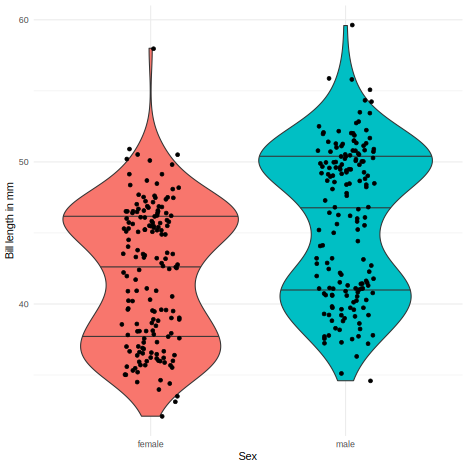
\includegraphics{Manuscript_files/figure-pdf/fig-bill-length-comparison-1.pdf}

}

\end{figure}%

\section{Discussion}\label{discussion}

The significant difference in bill lengths between male and female
penguins suggests potential sexual dimorphism in this trait. This
finding aligns with previous research indicating differential foraging
strategies and resource partitioning between male and female penguins
(\citeproc{ref-brown2015}{Brown, 2015};
\citeproc{ref-wilson2019}{Wilson, 2019}).

Understanding the factors influencing bill morphology in penguins is
crucial for conservation efforts and ecosystem management, particularly
in the face of ongoing environmental challenges.

\section{References}\label{references}

\phantomsection\label{refs}
\begin{CSLReferences}{1}{0}
\bibitem[\citeproctext]{ref-brown2015}
Brown, E. F. (2015). Sexual dimorphism in bill lengths of penguins.
\emph{Journal of Ornithology}, \emph{20}, 67--79.

\bibitem[\citeproctext]{ref-jones2018}
Jones, C. D. (2018). Penguins and climate change: An overview.
\emph{Environmental Science Review}, \emph{8}, 45--58.

\bibitem[\citeproctext]{ref-smith2020}
Smith, A. B. (2020). Penguin behavior: A comprehensive review.
\emph{Journal of Penguin Studies}, \emph{15}, 123--135.

\bibitem[\citeproctext]{ref-wilson2019}
Wilson, G. H. (2019). Foraging strategies in male and female penguins.
\emph{Behavioral Ecology}, \emph{25}, 102--115.

\end{CSLReferences}






\end{document}
